%
% Reproducibility manuscript: describe results from relative
% alchemical free energy simulation done with various MD packages.
%
% arara: make
% arara: pdflatex
% arara: bibtex
% arara: pdflatex
% arara: pdflatex
% arara: clean: {files: [reprod.aux, reprod.bbl, reprod.blg, reprod.log, acs-reprod.bib, reprod.lod, reprod.fls]}
%

\documentclass[journal=jctcce,manuscript=article]{achemso}

\usepackage[T1]{fontenc}
\usepackage{graphicx}
\usepackage{amsmath,amssymb,mathrsfs}
\usepackage{xr}
\usepackage{booktabs}
\usepackage{multirow}
\usepackage{rotating}
\usepackage{siunitx}
\usepackage{easy-todo}
\usepackage{footref}


\externaldocument[S-]{SI}

\sisetup{
  separate-uncertainty = true
}

\newcommand{\progname}[1]{\texttt{#1}}
\newcommand{\inpopt}[1]{\texttt{#1}}
\renewcommand{\footnoterule}{}
\renewcommand{\vec}[1]{\mathbf{#1}}


\title{Reproducing Relative Alchemical Free Energies of Hydration
  (draft)}

\author{Hannes H. Loeffler}
\affiliation[Scientific Computing Department, STFC]{Science \&
  Technology Facilities Council, Daresbury, Warrington, WA4 4AD,
  United Kingdom}
\email{Hannes.Loeffler@stfc.ac.uk} \phone{+44 1925 603367}

\author{Stefano Bosisio}
\affiliation[University of Edinburgh]{EaStCHEM School of Chemistry,
  University of Edinburgh, David Brewster Road, Edinburgh EH9 3FJ, UK}

\author{Guilherme Duarte Ramos Matos}
\affiliation[University of California, Irvine]{Department of
  Chemistry, University of California, Irvine}

\author{Donghyuk Suh}
\affiliation[University of Chicago]{University of Chicago}

\author{Julien Michel}
\affiliation[University of Edinburgh]{EaStCHEM School of Chemistry,
  University of Edinburgh, David Brewster Road, Edinburgh EH9 3FJ, UK}

\author{David L. Mobley}
\affiliation[University of California, Irvine]{Departments of
  Pharmaceutical Sciences and Chemistry, University of California,
  Irvine}

\author{Benoit Roux}
\affiliation[University of Chicago]{University of Chicago}


\keywords{Free Energy, Hydration, Alchemical, Reproducibility, Automation}



\begin{document}

\begin{abstract}
  Alchemical free energy calculations are an increasingly important modern simulation
   technique.  Contemporary Molecular Dynamics and Monte Carlo 
  software such as AMBER, CHARMM, GROMACS and Sire/SOMD include support for the 
  method.  Implementation details vary among those codes but users expect 
  reliability and reproducibility, i.e.\ a simulation must yield a comparable 
  free energy within statistical bounds regardless of code used.  
  \emph{Relative} alchemical free energy simulation has been less well tested 
  than its absolute counterpart.  However, relative transformations are thought to 
  be computationally and statistically more efficient.  Thus, reproducibility of computed 
  relative free energies across simulation packages is also crucial. Here we present the 
  results for relative alchemical free energy (RAFE) calculations for hydration free energies of a set of small 
  organic molecules and show that free energies can be satisfactorily 
  reproduced with aforementioned codes given some level of care and attention to detail.  We will also recommend simulation 
  protocols, setup procedures and analysis techniques, and we discuss what 
  needs to be done to ensure continued progress.
\end{abstract}

\begin{tocentry}
  % \includegraphics[scale=1.0]{}
\end{tocentry}

\todo{Objectives:
 Do the relative free energy results produced across different
 softwares agree with each other? What if they don't?}

\todo{Objectives:
 Can we outline what should be a standard procedure to calculate
 relative free energies of hydration alchemically?}

\todo{Objectives:
 We want to emphasize that we aim at improving codes/protocols/practices and not highlight "bad" codes
}

\todo{Be clear on what reproducibility means here e.g. no exact numerical}

\section{Introduction}
\label{sec:intro}

The free energy is a fundamental function of thermodynamics and
kinetics as it explains how processes in nature evolve.  The equilibrium balance of products and reactants in
a hypothetical chemical reaction can be immediately determined
from the knowledge of the free energy difference of reactants and
product and their concentrations.  The free energy landscape of a given system, however, can be
very complicated and rugged with barriers which impose
limits on how fast the process can take place.  It is therefore of
little surprise that the determination of this reversible work is of
utmost importance to all natural sciences e.g.\ for binding and
molecular association, solvation and solubility, protein folding and
stability, partition and transfer, and design and improvement of force
fields.

The calculation of free energies through
computers~\cite{hansen_practical_2014, doi:10.1021/jp102971x,
  Gallicchio201127, doi:10.1080/08927022.2015.1132317,
  doi:10.1146/annurev.matsci.32.111901.153708} has been particularly
attractive as it promises to circumvent certain limitations of experimental
approaches. Specifically, processes can be understood at the molecular and atomic level and 
there is the potential that computational techniques can be more cost and time effective.  Thus, a
multitude of methods have been devised to make reversible work
estimates accessible through computation~\cite{hansen_practical_2014,
  doi:10.1021/jp102971x, Gallicchio201127,
  doi:10.1080/08927022.2015.1132317,
  doi:10.1146/annurev.matsci.32.111901.153708}.  However, the
reliability of estimates is still very much a matter of
concern~\cite{doi:10.1021/jp102971x, doi:10.1021/acs.jctc.5b00179}.
Roughly speaking, fast methods tend to be less accurate while more
accurate methods tend to be slow.  Nevertheless, rigorous
methods are obligatory in obtaining accurate, precise and reliable
results, while less accurate methods can be used as an input filter
for more expensive approaches.  By rigorous we mean methods that give
asymptotically correct free energy estimates i.e. they are correct in the limit 
of sufficient simulation time.

One such method is the so-called \emph{alchemical} free energy
approach whose theory is firmly rooted in statistical thermodynamics
and is argued to be the most accurate method in quantitative
prediction of free energies~\cite{Beveridge-citeulike:3789890,
  straatsma:92, doi:10.1021/cr00023a004, hansen_practical_2014}.  The
method has been applied in various forms for many decades now since
the early days of computer simulation~\cite{doi:10.1063/1.1671118,
  bennett_efficient_1976, doi:10.1063/1.432264, FS9821700055,
  Tembe1984281, doi:10.1063/1.449208}.  The method has gained renewed
attention in recent years --- concomitant with improvements in
computer hardware design --- both within the traditional equilibrium
framework~\cite{GILSON19971047, doi:10.1021/jp0217839,
  deng_computations_2009} but also increasingly in combination with
non-equilibrium techniques~\cite{ytreberg_comparison_2006, JCC:JCC23804,
  doi:10.1021/ct500964e}.  The name comes from the nonphysical
intermediates that often need to be created to smoothly interpolate
between end states and because parts or all of a molecule may ``appear''
or ``disappear'' in a transformation.  In the context of force field
methods the transformation takes place in parameter space, i.e.\ the
force field's parameters determining strength and equilibrium of
interactions are varied by scaling.  This can be a particular
efficient approach as it does not require translocation in
configuration space.  For instance, the dissociation of a ligand from
a large biomolecule may involve many degrees of freedom while, at the
same time, it is generally unclear along which coordinates a
translocation simulation should take place.

Alchemical free energy simulations are constructed around the concept
of thermodynamic cycles~\cite{Tembe1984281}.  As the free energy is a state function, the sum of free energy changes
computed around any closed cycle must sum to zero.  This also implies
that the reversible work can be computed arbitrarily along
conveniently chosen legs of the cycle.  E.g.\ in
Fig.~\ref{fig:thermocycle} the relative free energy of hydration can
be computed along the vertical legs, that is, following the physical
process of moving a molecule from the gas phase to the liquid phase,
or along the horizontal legs in an nonphysical alchemical calculation.
As mentioned above, the latter may be computationally and
statistically more efficient.

\begin{figure}[ht]
  
\includegraphics[scale=1.0]{figures/thermocycle.pdf}
  \caption{The thermodynamic cycle to compute the relative free energy
    of hydration
    $\Delta\Delta G_{\mathrm{hydr}}=\Delta G_{\mathrm{sol}}-\Delta
    G_{\mathrm{vac}}=\Delta G'' - \Delta G'$.  The example is for the
    ethanol $\leftrightarrow$ methanol transformation.  Alchemical
    simulations can be performed along the non--physical horizontal
    legs while vertical legs illustrate the physical process (which is
    directly accessible through absolute alchemical free energy
    simulation, see e.g.\ Ref.~\citenum{doi:10.1021/acs.jced.7b00104}).}
  \label{fig:thermocycle}
\end{figure}

Absolute (standard) alchemical free energy calculation has been a
particular focus of recent years~\cite{GILSON19971047,
  doi:10.1021/jp0217839, deng_computations_2009,
  ytreberg_comparison_2006, doi:10.1021/ct500964e}.  \emph{Absolute}
here really means that the equilibrium constant of a physical
reaction, e.g.\ binding and dissociation, can be calculated directly
by completely decoupling a whole molecule from its environment and the
term is mostly being used to discriminate against \emph{relative}
techniques (see below).  Decoupling means the scaling of the non--bonded 
\emph{inter}--molecular interactions between the perturbed group (all atoms 
that differ in at least one force field parameter between the end states) and 
its environment.  We distinguish this from ``annihilation'' which would also
scale the \emph{intra}--molecular interactions in addition to the 
inter--molecular interactions. These schemes may require two 
simulations along the opposite edges of a quadrilateral thermodynamic cycle 
but approaches that produce the reversible work directly in one simulation
have been proposed too~\cite{doi:10.1063/1.3519057, C3FD00125C}.

Relative alchemical free energy (RAFE) calculations ``mutate'' one
molecule into another one.  This is most efficiently
achieved~\cite{doi:10.1021/j100056a020, Michel2010} by making use of
the single topology method~\cite{doi:10.1063/1.449208,
doi:10.1021/j100056a020, doi:10.1021/jp981628n}.  Single topology means that 
there is only one representation of the molecule to be mutated, also implying a 
single set of coordinates.
% Should we have a figure explaining the difference? In SI?
Thus, atom types are directly transformed into the new type,
typically by linearly scaling the force field parameters.
Disappearing/appearing atoms need to be balanced with ``dummy'' atoms to ensure 
constant number of atoms in both end states.  Dummy atoms have no non--bonded 
interactions in the end state but retain the bonded terms of the original atom 
to avoid complications with unbound atoms~\cite{doi:10.1021/jp981628n} (see 
also ``wandering'' ligand problem below).  AMBER is a special case
as it does not require the user to define dummy atoms explicitly, i.e.\ as 
atoms with coordinates and zero end state parameters in the topology, but only 
to mark the disappearing and appearing atoms in the control file for the 
MD engine.  The contributions of bonded terms that involve at least one 
dummy atom will not be factored into the free energy as it is assumed that 
those contributions will perfectly cancel in the thermodynamic 
cycle~\cite{doi:10.1021/acs.jcim.5b00057, doi:10.1021/jp994193s}.

RAFEs are useful for instance in ranking which one of a set of molecules binds 
strongest to a chosen target.  This approach has recently gained more traction 
in the context of relative free binding energies between small molecules e.g.\ 
drug or lead like molecules and biomolecules~\cite{doi:10.1021/ja512751q, 
doi:10.1021/acs.jctc.6b00991}.

The single topology approach~\cite{doi:10.1021/j100056a020} requires a
certain similarity between the two mutated states.  This means primarily
topological and structural similarity but also chemical similarity is
of importance e.g.\ chirality and binding modes where the relative
three dimensional arrangement in space must be taken into account.
Furthermore, ring breaking is technically
challenging~\cite{doi:10.1021/acs.jctc.6b00991} but it has also been
shown that this should be done only in certain
circumstances~\cite{doi:10.1021/acs.jcim.5b00057,
  doi:10.1021/jp994193s}.

When the two molecules are very dissimilar, the dual topology
method~\cite{doi:10.1021/j100056a020, doi:10.1021/jp981628n} can be
applied to compute relative free energies.  In this approach all atoms
in the end states are duplicated and thus both sets are present at all
times but don't interact with each other.  Only non--bonded
interactions need to be scaled such that the disappearing end state
corresponds to an ideal gas molecule~\cite{doi:10.1021/jp981628n}.
This, however, comes with additional complications as two independent
molecules can drift apart and so suffer from the ``wandering'' ligand
problem as in absolute transformations\cite{GILSON19971047,
doi:10.1021/jp0217839, deng_computations_2009}.  Topological
similarity can only be exploited when the charges of the common core
are explicitly made equivalent~\cite{doi:10.1021/acs.jctc.5b00179}.
This approach, however, shifts all the chemical variability
exclusively to the dummy atoms and is thus of only limited use.

Technically, a dual topology calculation is the same as two absolute
calculations run simultaneously in opposite directions.  It has been
shown though that with the introduction of special restraints or
constraints this can be a viable option~\cite{doi:10.1021/ct700081t,
  rocklin_separated_2013}.  A covalent link, e.g.\ as in side--chain
mutation simulations, provides a natural restraint such that dual
topology simulations can be applied without further problems.  Modern
MD software e.g.\ AMBER~\cite{case_amber_2005},
CHARMM~\cite{JCC:JCC21287}, GROMACS~\cite{Abraham201519},
GROMOS~\cite{doi:10.1021/jp984217f} and Sire/SOMD~\cite{Sire-2016,
  doi:10.1021/ct300857j} offer a hybrid single/dual topology approach
i.e.\ the user can specify which part of a perturbed group should be
handled by which method~\cite{doi:10.1021/jp994193s}.

As alluded to above, reliability is a principal matter of concern.  In
particular, we need to ensure reproducibility of free energy results
among computer codes.  To the best of our knowledge this has not been
systematically tested yet for a set of different MD packages. 
However, there have been some recent efforts to test \emph{energy} reproducibility across 
packages -- a necessary but not sufficient prerequisite [ref Shirts 10.1007/s10822-016-9977-1]
Given a
predefined force field and run--time parameters we should be able to
obtain comparable free energy results within statistical convergence
limits.  In practice, we have the problem, however, that the methods
and algorithms used in one MD program are not always present in another
package or are the same, such as algorithms for pressure and temperature scaling,
integrators, etc.  Nevertheless, the reversible work computed with any
simulation software should be expected to be reproducible within statistical error.  Modern MD
packages support a wide range of force fields and methods such that
these packages are replaceable with each other to an ever increasing
extent and the choice of the right package for the user becomes less
and less a matter of technical restrictions.

In this work we present the results of relative hydration free
energies of a set of small organic molecules (see
Fig.~\ref{fig:cycles}).  Solvation free energies have a wide range of
uses and various methods exist to compute
them~\cite{Skyner:2015:PCCP}.  They are also needed to calculate
binding free energies where the simulation in solution (see
Fig.~\ref{fig:thermocycle}) is combined with a mutation of the
molecule bound to a partner, and other important physical
properties~\cite{Skyner:2015:PCCP}.  A large database of hydration
free energies computed from alchemical free energy (AFE) simulation, FreeSolv, has been
presented recently~\cite{doi:10.1021/acs.jced.7b00104} and was just updated [ref 10.1021/acs.jced.7b00104]. Here, we are interested 
in the reproducibility of RAFE with the simulation programs AMBER, CHARMM,
GROMACS and Sire/SOMD.  We will discuss the reversible work results
obtained with these packages and make recommendations
regarding simulation protocols, setup procedures and analysis
techniques.  We will also deliberate on what needs to be done to progress the 
field, both from a usability perspective as well as from the view point of code 
development.


\section{Methods}
\label{sec:methods}

\subsection{Alchemical Free Energy Implementations}
\label{sec:afe_impl}

We begin by describing the differences in the alchemical free energy
%DLM: "working out"? Unclear if this means "finding" or "describing" which are rather different; I think we mean "describing"
implementations of the four MD codes AMBER, CHARMM, GROMACS and
Sire/SOMD.  One key difference is in the softcore
functions employed~\cite{beutler_avoiding_1994,
  zacharias_separationshifted_1994} used in each code as summarised in
section~\ref{S-sec:softcores} of the SI.  Softcore functions are used to avoid numerical and thus
stability problems of the conventional van der Waals and Coulombic
potentials~\cite{steinbrecher_nonlinear_2007} as they have
singularities at zero distance (vertical asymptotes).  Direct scaling
of these potentials causes the functions to increasingly behave like
hard--sphere potentials as $\lambda\rightarrow 0$.  This implies a
higher probability of other atoms to penetrate into the highly
repulsive short--range portion of the potential which can lead to
strongly fluctuating forces/energies and to severe instabilities in
the integrator, as well as analysis problems even when simulations run~\cite{beutler_avoiding_1994,
  zacharias_separationshifted_1994, steinbrecher_nonlinear_2007}.

Other differences include whether the code scales individual (force field)
parameters and/or the total energy~\cite{doi:10.1021/jp981628n}, or if
%DLM: What does it mean to scale the total energy? Can you be more clear? I'm assuming what you mean is that in some cases, one actually modifies the force field parameters, whereas in others, one modifies the contributions of those terms to the potential energy/total energy by scaling those terms in the Hamiltonian?
%DLM: Also, after reading below -- do we need to define one of these approaches as "energy scaled"? We don't introduce the term "energy scaled" but we use it below
the code allows constraints for bonds with changing bond lengths.
These and other details will be outlined below.  The perturbed group
consists of all atoms that need to be transformed, i.e.\ any atom
that differs in at least one force field parameter in the other end
state.

\paragraph{AMBER} This code is strictly dual topology and all terms
are energy--scaled.
%DLM: See above, what is "energy--scaled"?
  The code allows, however, mapping of atoms in a
single topology fashion and computes the forces appropriately
(linearly) scaled for each atom in the pair. 
%DLM: Why is "appropriately" "linearly" here? This would presumably apply only to non-softcore terms? Somewhat confusing to say it this way then...?
The perturbed group must
be entirely duplicated i.e.\ for \progname{sander} this means two topology files
with one end state each, and for \progname{pmemd} both end states in one topology
file.  The softcore potential applies to any atom chosen by the user i.e.\ also 
for atoms that have an equivalent in the other state but non--softcore atoms 
must still match 1:1 in both states.  Explicit dummy atoms are 
not needed as the code will only compute bonded contributions for ``real''
atoms and thus ignores bonded energies involving dummy atoms (implicit dummy 
%DLM: I think this is defining the term "implicit dummy protocol" for the first time; it could be made more clear, as I just read right past it and later when I encountered the term again, I wondered, "what is the implicit dummy protocol?"
protocol).  The code cannot handle constraints of changing bond lengths in the 
perturbed group.
%DLM: "changing bond lengths involving constraints" perhaps more clear? 
  There is only one global $\lambda$ for parameter 
transformation.  Separated protocols (see below) must be emulated through 
careful construction of topologies by keeping force field parameters that are not being modified constant 
between different files.

\paragraph{CHARMM} The PERT module duplicates the topology similar to
\progname{sander} but the data structures for mapped atoms are present only once.  The
%DLM: What does it mean for the "data structures" to be present only once? Maybe something like, "definitions for mapped atoms are given only once"? 
%DLM: Can we provide sample files for all of these in SI, and maybe even give topology snippets in figure(s) to illustrate the point? 
module requires balancing with explicit dummy atoms.  All terms are
energy--scaled.  The PSSP softcore potential is applied to \emph{all}
atoms in the perturbed group (see section~\ref{S-sec:softcores} in the SI).  The code can handle
constraints of changing bond lengths in the perturbed group but this
may cause wrong results with PSSP softcores (Stefan Boresch, private
communication).  There is only one global $\lambda$ for parameter
transformation, however, the scripting facilities allow run time
%DLM: What scripting facilities? 
modification of topologies e.g.\ by setting charges or vdW parameters
to arbitrary values.

\paragraph{GROMACS} This code uses a single topology description.
Bonded terms are strictly parameter--scaled which requires proper
%DLM: Need to define "parameter--scaled"
balancing of multi--term dihedrals.  Non--bonded terms are
energy--scaled.  The softcore potential applies to dummy atoms only
determined from atoms having zero vdW parameters.  The code
allows changing bond lengths involving constraints within the perturbed group but
this can lead to instabilities and wrong results (Michael Shirts,
private communication).  There are separate $\lambda$s for vdW,
Coulomb and bonded parameters (and some other).
%DLM: The other sections discuss the possibility of separated protocols; this probably should be addressed explicitly here (e.g. "Separated protocols are possible here because there are separate $\lambda$s...")

\paragraph{Sire/SOMD} This code uses a single topology description.
The final state is constructed at run time from the initial state with
a ``patch'' (list of force field parameters to be modified).  Bond and
angle terms are parameter--scaled while all other terms are
energy--scaled.  The softcore potential applies to dummy atoms only.
The code cannot handle constraints of changing bond lengths in the
perturbed group.  There is only one global $\lambda$ for parameter
scaling.  Separated protocols (see below) must be emulated through
careful construction of the patch file.  Sire/SOMD is
Sire~\cite{Sire-2016} employing OpenMM~\cite{doi:10.1021/ct300857j}
for MD simulation.

\subsection{RAFE Setup}
\label{sec:rafe_setup}

The setup for all relative free energy simulations has been carried
out with the tool FESetup~\cite{loeffler_fesetup:_2015} in version
1.2.  FESetup is a perturbed topology writer for AMBER, CHARMM,
GROMACS, Sire/SOMD and also NAMD~\cite{JCC:JCC20289} (within the
limits of the dual topology approach).  The tool makes use of a
maximum common substructure search algorithm to automatically compute
atoms that can be mapped i.e.\ atoms that have a direct relationship
to an equivalent atom in the other state.  This means atom type to
atom type conversion and the only current limit is that rings are
required to be preserved~\cite{doi:10.1021/acs.jcim.5b00057}.  In this
way we achieve a maximal single topology description: any atom that
does not match will be made a dummy atom.  FESetup allows
equilibration of the solvated simulation systems and ensures that
``forward'' and ``backward'' simulations will have the same amount of
total atoms.  The tool creates all input files with control
parameters, topologies and coordinates as required for RAFE
simulations.  Full details on FESetup can be found in
Ref.~\citenum{loeffler_fesetup:_2015}.

Figure~\ref{fig:cycles} shows all 18 transformation considered in this
study including ``forward'' and ``backward'' mutations.  RAFE
simulations are principally fully symmetric i.e.\ they do not have a
directionality with respect to the coupling (order) parameter
$\lambda$.  Performing simulations in either direction, however, is
applied here as a test for possible discrepancies.
%DLM: I don't understand what it means for them to be "principally fully symmetric".
%DLM: I also think it may confuse the reader to say that the directionality doesn't matter but that you do tests in both directions; maybe
% you want to explain what exactly this is testing then. 

\begin{figure}[ht]
  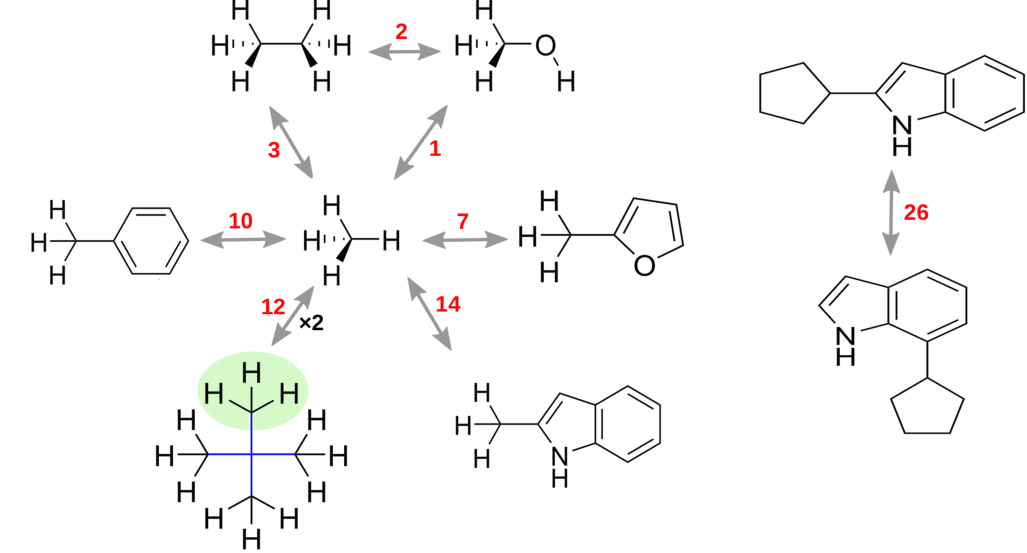
\includegraphics[scale=1.0]{figures/cycles.pdf}
  \caption{The thermodynamic cycles considered in this study.  To
    compute the free energy of hydration all pair--wise
    transformations have to be carried out once in solution and once
    in vacuum.  Green and blue colours in neopentane show two
    alternative mappings for methane.  The numbers in red denote the
    number of dummy atoms.}
  \label{fig:cycles}
\end{figure}
%DLM: Hannes, would you mind depositing PDFs with the figures compiled? I still haven't been able to get the figures to compile properly locally, so it'd be really useful if I could read a PDF that has the figures. :) 

The ethane $\rightarrow$ methanol transformation is traditionally
regarded as a standard test for RAFE
simulations~\cite{doi:10.1063/1.449208, doi:10.1021/jp981629f}.  The
other transformations are centred around mutations from and to
methane.  The 2--cyclopentanylindole to 7--cyclopentanylindole
transformation has been added to include both deletion as well as
insertion of sub--parts of the perturbed group in one simulation.  For
neopentane $\rightarrow$ methane we point out that there are two
alternative mappings possible, see Figure~\ref{fig:cycles}.  One in
which methane is mapped with a terminal methyl (green) and the other
one where the methane carbon is mapped with the central carbon in
neopentane (blue).  Results from both mutations will be shown and
discussed.


\subsection{RAFE Simulation Protocols}
\label{sec:rafe_protocols}

One of the major concerns in a reproducibility study is to ensure
consistency in the applied protocols.  This is complicated by the fact
that MD software employs a wide range of methods and algorithms that
may not be available in the other MD software.  For example, pressure and
temperature scaling, integrators and other algorithms can be very
different.  It is also unclear if and how implementation details can
affect results, in particular see subsection~\ref{sec:afe_impl} discussing the 
implementation details of alchemical free energy simulation in code.

In this study we look at a set of simple organic molecules (see
Figure~\ref{fig:cycles}).  As the focus here is on probing for
reproducibility among various MD packages, we chose fairly small,
rigid and neutral molecules to keep problems with sampling low, and
avoid difficulties with charged
particles~\cite{rocklin_calculating_2013, JCC:JCC1050}.  The force
field was chosen to be GAFF~\cite{wang_development_2004} (version
1.8), utilising AM1/BCC charges~\cite{jakalian_fast_2000,
  jakalian_fast_2002} for the solute and
TIP3P~\cite{jorgensen_comparison_1983-1} for the solvent.  The quality
of free energies of various small molecule force fields has been shown
elsewhere, see e.g. Refs.~\citenum{doi:10.1021/ct300203w,Hu2016}.
%DLM: Can we say how charges were assigned? Antechamber?

While the MD packages principally allow a ``one--step'' 
transformation~\cite{steinbrecher_soft-core_2011}
that is both van der Waals and Coulombic contributions vary
simultaneously, it can be(is? ref?) more efficient to carry out a
separated protocol.  In such a protocol the charges are transformed
linearly between the end states followed by a mutation of the van der
Waals parameters using a softcore
potential~\cite{beutler_avoiding_1994,
  zacharias_separationshifted_1994} (see section~\ref{S-sec:softcores} in the SI for details) on the vdW
term only.  It is important to note that in the separated protocol
charges have to be switched off before vdW parameters (and vice versa
for the transformation in opposite direction) to avoid collapse of
other atoms, e.g. solvents, onto a ``naked'' charge, see 
section~\ref{S-sec:separated} in the SI.
%DLM: I think there is a literature reference on the need to do this; asking Guilherme for it as I don't recall it off the top of my head.

All simulations were started from the simulation box pre--equilibrated with
FESetup~\cite{loeffler_fesetup:_2015}.
%DLM: This seems to be saying that the box is pre-equilibrated with FESetup? Is that really what you mean, or do you mean a simulation box prepared with FESetup and then pre-equilibrated? Or a pre-equilibrated simulation box then prepared with FESetup?
  It should be noted, however, that in
constructing the system steric overlaps between the solute and the solvent can
happen.  This is because the number of atoms are always chosen to be the same
%DLM: Not following how this can happen if it is pre-equilibrated. Do you mean it was pre-equilibrated BEFORE adding the solute, or pre-equilibrated for just one lambda value, or ... ? Would be helpful to be slightly more specific.
for forward and backward setups by using the larger box of the two.  Thus, in
transformation from a smaller to a larger solute water molecules may be in
close distance.  The simulations were run at \SI{298.15}{K} and \SI{1.0}{bar}.

\paragraph{AMBER} The starting coordinates were usually taken directly from the
pre--equilibrated setup step but no further $\lambda$ specific equilibration 
was carried out, i.e.\ RAFE MD simulations were started with new velocities appropriate for the 
final simulation temperature.  In a very few cases it was necessary to use 
coordinates from a nearby $\lambda$ state because of simulation instabilities.  
This happened in transformations with a larger number of dummy atoms.  Water 
hydrogens (TIP3P) were constrained with SHAKE but none of the atoms in the 
perturbed group
%DLM: I think it should be "constrained with SHAKE, as were all bonds involving hydrogen except those within the perturbed group. None of the bonds in the perturbed group were constrained." Is that right? (Currently, you say you don't constrain within the perturbed group but you don't say that you DO constrain the other ones, which is odd.)
 and so the time step was set to \SI{1}{fs} (see Sire protocol 
below for an alternative approach).  The temperature was controlled through a 
Langevin thermostat and pressure through a Monte Carlo barostat.
%DLM: For consistency with Sire/SOMD (and thoroughness) we should give details of friction constant/pressure rescaling.


\paragraph{Sire/SOMD} All simulations were carried out with
Sire/OpenMM 6.3 (revision 16.1).  Each alchemical transformation was
divided into 17 evenly spaced windows and simulated for \SI{2}{ns}
both in water an vacuum phase. A velocity-Verlet integrator was
employed with \SI{2}{fs} timestep, constraining all the hydrogen bonds
not alchemically transformed (unperturbed H protocol).
%DLM: It's not clear what "unperturbed H protocol" refers to; are we introducing a new term? 
 An atom--based
Barker--Watts reaction field~\cite{doi:10.1080/00268977300102101} with
a dielectric constant of \num{82.0} was adopted for water phase
simulations. Furthermore, a cutoff of \SI{12}{\angstrom} was set for non-bonded
interactions and periodic boundary conditions were imposed.
Temperature control was achieved with the Andersen
thermostat~\cite{doi:10.1063/1.439486} with a coupling constant of
\SI{10}{ps^{-1}}.  A Monte Carlo barostat assured pressure control,
attempting isotropic box edge scaling every 25 time steps.
The reaction field was not employed in vacuum
and a Coulombic potential without cutoff was used.
This aspect led to an inconsistent description of the intramolecular electrostatic interactions
of the solute in the solvated and vacuum phases.
Thus, to enable a meaningful estimation of the free energy change 
a free energy correction term $G_{\mathrm{FUNC}}$ was
evaluated to treat intramolecular Coulombic interactions consistently
between water and vacuum legs of the thermodynamic cycle, fig~\ref{fig:thermocycle}, as explained
in ~\cite{Bosisio2016} . The $G_{\mathrm{FUNC}}$ term was obtained
via post-processing the end states trajectories of each water
phase simulation, using the Zwanzig relationship~\cite{zwanzig_high-temperature_1954}:
\begin{equation}
 \label{eq:ZwanzigDGfunc}
 G_{\mathrm{FUNC}} = -\beta^{-1} \ln \langle exp \left[-\beta(U_{\mathrm{ic,nc}}(\mathbf{r}) - U_{\mathrm{ic,sim}}(\mathbf{r}))\right]\rangle_{\mathrm{sim}}
\end{equation}
where $U_{\mathrm{ic,nc}}(\mathbf{r})$ is the solute intramolecular electrostatic 
potential that depends on the coordinates $\mathbf{r}$ of the solute and is given by Coulomb's law. 
$U_{\mathrm{ic,sim}}(\mathbf{r})$ is the intramolecular electrostatic potential term as
computed in the simulation with a BWRF cutoff. 

\paragraph{GROMACS} We used GROMACS 4.6.7 to carry out simulations for 
the relative hydration free energies ($\Delta \Delta G_{\mathrm{hydr}}$).
Each transformation had its Gibbs free energy calculated: (i) in a single topology 
approach in which van der Waals energy terms were changed separately 
from the electrostatic and bonded components; (ii) in a single topology approach in which  
bonded, van der Waals, and electrostatic terms are changed together;  and (iii) via the difference 
between two absolute calculations.
In the first two cases, each alchemical transformation was described by 31 and 16 
states, respectively, and simulated for 4.2 ns with time steps of 1 fs in water and a vacuum. 
Atomic masses were not changed along the alchemical path;
their change affect kinetic energy only and do not contribute for the free energy change. 
We used the Langevin integrator implemented in GROMACS with default friction 
coefficient of 1.0 $ps/ m_{atom}$. 
Absolute hydration free energies were calculated using a protocol used in previous works \cite{duarte_ramos_matos_approaches_2017, mobley_freeSolv:_2014}.
A Parrinello-Rahman barostat with $\tau_p =$ 10 ps and compressibility equal to 4.5 $\cdot 10^{-5}$ bar$^{-1}$.
We used two methods to calculate electrostatic interactions: Particle Mesh Ewald (PME) 
and Reaction Field with a dielectric of 78.3, as implemented in the software. 
We set the non-bonded cutoff to 10 angstroms, with a switch starting at 9 angstroms. 
PME calculations were of order 6 and had a tolerance of 1.0 $\cdot 10^{-6}$, with a grid spacing of 1 angstrom. 
All transformations required the use of soft-core potentials to avoid numerical problems in the free energy calculation. 
We chose the 1-1-6 soft-core potential for Lennard-Jones 
terms and used the default soft-core Coulomb implementation in paths where charges, van der 
Waals, and bonded terms were modified together, but no soft core potentials were applied 
to Coulomb interactions when Coulomb interactions were modified separately.

\todo{make figure explaining the protocols described here.}

\subsection{Analysis}
\label{sec:analysis}

Various estimators have been proposed to obtain the free energy from AFE 
simulations.  Early work by Kirkwood~\cite{kirkwood_statistical_1935} expresses 
the free energy as an ensemble average of the derivative of the
Hamiltonian with respect to the coupling parameter $\lambda$.  The
method is now known as Thermodynamic Integration (TI).  Zwanzig
devised the exponential formula~\cite{zwanzig_high-temperature_1954}
(EXP), also known as Free Energy Perturbation (FEP) or thermodynamic
perturbation (TP), which calculates the free energy from the
exponential average of the energy difference of the end states.  The
energy difference is computed with the configuration of one end state
being used for both end states assuming that this configuration is
representative for either state.  As the phase--space overlap needs to
be sufficiently large~\cite{wu_phase-space_2005,
  wu_phase-space_2005-1} the EXP approach typically needs
intermediates, controlled by $\lambda$.  However, it has been shown
that EXP has an asymmetric bias depending on the directionality of
$\lambda$~\cite{wu_asymmetric_2004} and that the Bennett Acceptance
Ratio (BAR) method~\cite{bennett_efficient_1976} is considerably more
effective in obtaining an accurate result~\cite{lu_appropriate_2003}.
BAR is a generalization of EXP by making explicit use of the
``forward'' ($\lambda_i \rightarrow \lambda_{i+1}$) and ``backward''
($\lambda_{i+1} \rightarrow \lambda_i$) estimates.  Later it was
demonstrated that this can be effectively extended to incorporating
more than just the immediate $\lambda$ neighbours and, in fact, all
other $\lambda$s.  This approach has been called multi--state BAR
(MBAR)~\cite{shirts_statistically_2008-1} method.  MBAR has been shown
to have the lowest variance of any known
estimator~\cite{shirts_statistically_2008}.

In this work we primarily focus on TI as this is supported by all MD
packages ``out--of--the--box'', whereas BAR and MBAR are not.
Equation~\ref{eq:ti} computes the free energy as
\begin{equation}\label{eq:ti}
	\Delta G = \int_{\lambda=0}^{\lambda=1}
	\left\langle \frac{\mathscr{H}(\vec{q},\vec{p};\lambda)}{\partial\lambda}\right\rangle_\lambda d\lambda
\end{equation}
where $\mathscr{H}(\vec{q},\vec{p};\lambda)$ is the Hamiltonian as a function of the coordinate vectors $\vec{q}$ and the momentum vectors $\vec{p}$, and parametric dependence on the coupling parameter $\lambda$.  The angle brackets denote the ensemble average of the gradient of the Hamiltonian with respect to $\lambda$ at a given $\lambda$ value.  An AFE simulation is typically carried out in a series of equilibrium simulations at discrete values of $\lambda$ but the gradient can also be evaluated with a continuously varying coupling parameter as a function of the simulation time.  The free energy is finally computed through a suitable numerical integration method.

Results from additional estimators
will be given where available.  We have used the alchemical analysis
tool~\cite{klimovich_guidelines_2015} for all free energies.  This
tool provides various estimators such as TI, TI with cubic splines,
BAR and MBAR.  All data can be sub--sampled to eliminate correlated
data.

All RAFE simulations were run in triplicate in forward as well as
backward direction for a total of 6 simulations per mutation.  The
final hydration free energy $\Delta\Delta G_{\mathrm{hydr}}$ was
computed as the average for each direction separately.  For comparison we have also
calculated the absolute (standard) hydration free energies for all
molecules in Figure~\ref{fig:cycles}.
%DLM: Explain that these are less implementation-dependent and provide a check/"gold standard" set of answers? 

To estimate the reliability and convergence of the results, the
standard error of the mean (SEM) has been calculated.  The SEM is
defined as

\begin{equation}
  \label{eq:sem}
  \mathrm{err}(\Delta\Delta G_{\mathrm{hydr}}) = \frac{\sigma}{\sqrt{n}}
\end{equation}

where $\sigma$ is the sample standard deviation and $n$ is the size of
the uncorrelated sample.  The SEM for component free energies is combined as

\begin{equation}
  \label{eq:sem-comb}
  \mathrm{err}(\mathrm{combined}) = \sqrt{\sum_i \sigma_i^2}.
\end{equation}

which is appropriate if the property to be computed is a sum of
contributions.


\section{Results}
\label{sec:results}

\todo{what protocols did not work}

\subsection{AMBER}
\label{sec:amber-results}

Using AMBER for RAFE simulations has revealed several problems with
the implementation.  Some bugs were identified and have been fixed
by the developers, e.g. energy minimization in \progname{sander} led to diverged
coordinates for mapped atoms which is, however, a necessary condition
for a single topology description. %DLM: This reads like diverged coordinates is necessary, but I think you mean that consistent coordinates is necessary? 
%DLM: Also, should list what version of AMBER this was fixed for. 
 Other issues are that vacuum
simulations have to be carried out separately with the \progname{sander} program %DLM: Separately from what? Do you mean that if the solution calculations are done with PMEMD you have to do the vacuum calculations with sander anyway?
because \progname{pmemd} cannot handle AFE simulations in vacuum at the moment.  This will, however, be rectified in future versions (Ross Walker, private communication).  A disadvantage of \progname{sander} is that it cannot be used to simulate the $\lambda$ end points~\cite{doi:10.1021/ct400340s} such that the TI gradients need to be extrapolated (minimum and maximum allowed $\lambda$s are 0.005 and 0.995). 
%DLM: Wait, so this means that there's no way around extrapolating the endpoints in vacuum?
 Also, \progname{sander} considers the whole system as the perturbed
region while \progname{pmemd} restricts this to a user chosen atom selection.  This
has obvious implications for performance~\cite{doi:10.1021/ct400340s}.

We also found that, in contrast to the other three codes, AMBER cannot
correctly reproduce relative free energies in a 1--step protocol i.e.\
when all force field parameters are scaled simultaneously (see Table~\ref{S-tab:amber-onestep}).  This appears to be a problem when more than a few dummy atoms are involved while the 1--step protocol works for the smaller transformations (refer to Figure~\ref{fig:cycles}).  The separated RAFE protocol and absolute free energies, however, are very close to the other MD packages as demonstrated in Table~\ref{tab:amber-comp}.

End point geometries appear to be another issue with AMBER simulations
in both solution and vacuum.  This is most obvious in the neopentane $\rightarrow$ methane test case (central mapping).
%DLM: First use of the term "central mapping". What does it mean? 
  As shown in Figure~\ref{S-fig:amber-dist} the methane end state exhibits incorrect distances (which are too long) between the carbon and the four attached hydrogens of approximately \SI{1.23}{\angstrom}.  This value is about \SI{1.12}{\angstrom} for the terminal dummy atoms in the other test cases but still higher than the expected \SI{1.09}{\angstrom} on average.  Figure~\ref{S-fig:amber-dist} demonstrates how this depends on the number of dummy atoms immediately surrounding the central atom.
%DLM: I think we need error bars on the values otherwise it's impossible to tell if the difference is significant. 

We also compare free energies obtained from the implicit dummy approach in 
AMBER with results form explicit dummy atom simulations and results from 
absolute transformations.  Table~\ref{tab:amber-comp} lists the free energies 
for these three approaches together with the SEM.  SHAKE was explicitly 
deactivated for all bonds in the perturbed region in these protocols.
\begin{table}[]
  \begin{minipage}{\linewidth}
  \caption{Comparing AMBER results for simulations with implicit and explicit 
  dummy atoms, and results from absolute transformation.  A few select cases 
  with SHAKE enabled and a time step of \SI{2}{fs} are shown in addition.  
  Simulations were carried out with the separated protocol.  Signs of the 
  backward transformation have been reverted to correspond to the forward 
  transformation.}\label{tab:amber-comp}
  \makebox[\textwidth][c]{
  \begin{tabular}{llrrrr}
    \toprule
    &                & implicit & explicit & absolute & SHAKE\footnote{implicit 
    dummy atom protocol with $\delta t =$ \SI{2}{fs} and SHAKE on all H--bonds 
    except perturbed bonds.} \\
    \multicolumn{2}{l}{transformation}          & $\Delta\Delta G$  & 
    $\Delta\Delta G$ & $\Delta G$ & $\Delta\Delta G$ \\
    \midrule
ethane & methane & \num{0.02+-0.01} & \num{-0.13+-0.02}
&\multirow{2}{*}{\num{-0.02+-0.01}} & \\
methane & ethane & \num{0.00+-0.03} & \num{-0.19+-0.03} & & \\
methanol & methane & \num{6.19+-0.01} & \num{6.20+-0.02} & 
\multirow{2}{*}{\num{6.20+-0.01}} \\
methane & methanol & \num{6.20+-0.03} & \num{-6.15+-0.01} & & \\
ethane  & methanol & \num{-6.20+-0.01} & \num{-6.27+-0.01} &
\multirow{2}{*}{\num{-6.22+-0.01}} & -6.20 \\
methanol & ethane & \num{-6.20+-0.01} & \num{-6.25+-0.01} & & \\
toluene & methane & \num{3.24+-0.02} & \num{3.39+-0.02} &
\multirow{2}{*}{\num{3.19+-0.01}} & 3.29 \\
methane & toluene & \num{3.42+-0.03} & \num{3.52+-0.03} & & \\
neopentane\footnote{\label{foot:cent}central mapping.} & methane & 0.32 $\pm$ 
0.04 & \num{-0.03+-0.06} & \multirow{4}{*}{\num{-0.13+-0.02}} & 0.37 \\
methane\footref{foot:cent} & neopentane & \num{0.25+-0.03} & \num{-0.07+-0.03} & & \\
neopentane\footnote{\label{foot:term}terminal mapping.} & methane & \num{-0.13+-0.01} & \num{-0.12+-0.02} & & \\
methane\footref{foot:term} & neopentane & \num{-0.13+-0.03} & \num{-0.12+-0.03} & & \\
2-methylfuran  & methane & \num{3.09+-0.01} & \num{3.10+-0.01} &
\multirow{2}{*}{\num{2.96+-0.02}} \\
methane & 2-methyfuran  & \num{3.10+-0.03} & \num{3.15+-0.03} & & \\
2-methylindole & methane & \num{8.78+-0.03} & \num{8.78+-0.04} &
\multirow{2}{*}{\num{8.72+-0.01}} \\
methane & 2-methylindole & \num{9.14+-0.02} & \num{9.13+-0.03} & \\
2--cyclopentanylindole\footnote{\label{foot:partial}partial re/discharge i.e.\ 
only the charges of the appearing and the disappering 5--rings are switched.} & 
7--cyclopentanylindole & \num{0.36+-0.03} & \num{0.63+-0.06} & 
\multirow{2}{*}{\num{0.39+-0.04}} \\
7--cyclopentanylindole\footref{foot:partial} & 2--cyclopentanylindole & \num{0.34+-0.05} & \num{0.50+-0.03} & & \\
    \bottomrule
  \end{tabular}
}
  \end{minipage}
\end{table}
In addition, the table also shows selected results for transformations with 
SHAKE enabled for all bonds to hydrogens except those bonds that change bond 
length during transformation.  These free energies are computed from a single 
run as we generally observe very small SEM and in practice one simulation is 
sufficient to obtain converged free energy averages for all the systems studied 
here.  The time step has been increased from \SI{1}{fs} as used in the other 
three protocols to \SI{2}{fs}.  As the results are essentially the same as the 
non--SHAKE simulations, this SHAKE protocol appears to be a viable solution to 
increase the performance of RAFE simulations (cmp.\ SOMD simulations).  From a 
practical point of view, 
%DLM: How much speed difference does this make?
AMBER uses an atom based mask for bond SHAKEs such that the mask must be set 
for the hydrogens in question while the same is not possible for their 
counter--part in the other state because \emph{all} bonds emanating from this 
atom would be affected.

We can also compute the cycle closure error from Table~\ref{tab:amber-comp} for the closed cycle ethane$ \rightarrow$ methanol $\rightarrow$ methane $\rightarrow$ ethane (see Figure~\ref{fig:cycles}).  The free energy difference within a closed thermodynamic cycle must necessarily be zero.  For the implicit dummy simulation we calculate a cycle error for $\Delta\Delta G_\mathrm{hydr}$ of \SI{0.069+-0.041}{kcal.mol^{-1}} and for the explicit dummy simulation the error is \SI{-0.016+-0.047}{kcal.mol^{-1}}.

In general, the free energies computed with each approach are in good agreement with each other and with the results of the other MD packages.  There are, however, a few notable deviations.  Neopentane $\rightarrow$ methane with central mapping differs from the result with terminal mapping by about \SI{0.4}{kcal.mol^{-1}} (cf.\ Table~\ref{tab:amber-comp}). 
%DLM: first use of the term "terminal mapping" (except in the table). What does it mean? 
 The terminal mapping and the free energies from the explicit dummy simulations are, however, consistent with the absolute transformations.  We also observe a systematic deviation between forward and backward vacuum transformations in particular in the 2--methylindole simulation (see Table~\ref{S-tab:amber-disc}).
A discrepancy of consistently 0.2--\SI{0.4}{kcal.mol^{-1}} is evident from every $\lambda$ step of the vdW plus bonded transformation with both implicit and explicit dummy atoms).


\subsection{CHARMM}
\label{sec:charmm-results}

\todo{bug in TI gradient accumulation in parallel runs (does not affect
	serial?, does not affect EXP)}

\todo{cannot handle LRC: test with larger cutoffs and/or LRC correction
	with arbitrary, single structure; check http://pubs.acs.org/doi/abs/10.1021/jp0735987}

\subsection{GROMACS}
\label{sec:gromacs-results}

\todo{investigate why methane~ethane and ethane~methane differ so much from the other packages}

\todo{Make a figure that illustrates the choices of relative transformation}

\todo{Run split protocol simulations with gaff1.8 \textbf{\emph{and}} soft-core coulomb}

\todo{make figures XX1 and XX2 (I think they should probably go in the SI)}

GROMACS has some run input options which can simplify the procedure for setting up 
free energy calculations; however, these same options can also provide a source of error
if used naively. Additionally, running the simulations depends on understanding how these 
features are used because they can be a source of errors if misused. Specifically, 
\inpopt{couple-moltype} implicitly defines the initial and final states by giving a special tag
to a molecule and controls whether intramolecular interactions of the tagged molecule are 
retained or not along the alchemical path.
It should be used in absolute free energy calculations to tag the molecule which will be 
decoupled from the rest of the system. \inpopt{couple-moltype} should not be used in 
relative transformations in GROMACS because relative calculations rely on turning off 
interactions between only part of a molecule and the rest of the system, not the entire 
molecule. 
\inpopt{couple-lambda0} and \inpopt{couple-lambda1} control the interactions of the molecule
specified by \inpopt{couple-moltype} with its surroundings. For instance, if \inpopt{couple-lambda0}
is set to \inpopt{vdw-q} and \inpopt{couple-lambda1} to \inpopt{none}, the calculation will be set
in such a way that the tagged molecule is fully coupled to its surrounding by its electrostatic and
van der Waals interactions, while it will be completely decoupled from its surroundings in
the final state, effectively acting as an ideal gas molecule. These should be the default choices in
absolute free energy simulations; there is no need to specify both end states in the topology file.
In relative free energy calculations, however, \inpopt{couple-lambda0} and \inpopt{-lambda1} are
not necessary because \inpopt{couple-moltype} should be set to \inpopt{none}. 
\inpopt{couple-intramol} specifies if you want to modify intramolecular interactions along the alchemical 
path and should be set to \inpopt{yes} in relative transformations. Setting this to \inpopt{no}
would mean intramolecular interactions are maintained at their existing values while the 
free energy transformation is conducted, leading to an incomplete transformation and introducing 
errors in computed free energies.

Here, we choose absolute hydration free energies as our standard point of comparison 
because these are easily calculated with considerable precision \cite{duarte_ramos_matos_approaches_2017} %check for more references 
and are considerably simpler to set up and implement than relative calculations.
Prior work actually compared calculated absolute hydration free energies across different codes with considerable success \cite{klimovich_predicting_2010} (see Fig 7 in reference), further supporting this view.
Thus, we compared relative free energies calculated via simultaneous parameter change simulations -- our ``unified protocol'' -- 
and separated parameter change simulations -- our ``split protocol''-- to relative free energy 
calculations obtained from two absolute hydration free energies -- our ``absolute protocol''.
The unified protocol changes partial charges, van der Waals parameters, and bond 
parameters simultaneously along the alchemical path, while the split protocol 
stages the transformation in a van der Waals parameter change followed by a simultaneous  
bonded terms and charges modifications, or vice-versa. In the framework 
of the split routine, windows without a reasonably strong counterbalancing Lennard-Jones 
component are subject to very large electrostatic forces that will often lead to simulations
which crash with standard protocols~\cite{pitera_comparison_2002, anwar_robust_2005}.  
Thus we find that for stable and effective relative free energy calculations, particle deletion processes
require electrostatic terms to be turned off before van de Waals and bonded parameters are removed/modified. 
Insertion processes, in their turn, demand bonded and van der Waals parameters to be changed before charges are turned on.
The relative free energies of processes $A \rightarrow B$ and $B \rightarrow A$ tend to be equivalent if the protocol of the former
is the reverse of the latter, i.e., both end states should be connected by the same path in $\lambda$-space. 

\begin{sidewaystable}[]
\centering
\caption{Relative hydration free energies obtained from GROMACS simulations in $kcal\cdot mol^{-1}$.}
\label{tab:groresults}
\resizebox{\columnwidth}{!}{%
\begin{tabular}{llcccccccccccc}
\toprule
 &  & Split \footnote{\label{foot:split} results obtained from alchemical transformations with electrostatic and bonded scaling separate from vdW parameter change.} &  &  &  & Unified \footnote{\label{foot:uni} results obtained from alchemical transformation with all parameters scaling together.} &  &  &  & Absolute \footnote{\label{foot:abs}results obtained from absolute free energy calculations.} &  &  &  \\
 &  & GROMACS (RF) &  & GROMACS (PME) &  & GROMACS (RF) &  & GROMACS (PME) &  & GROMACS (RF) &  & GROMACS (PME) &  \\
Transformations &  & $\Delta \Delta G$ & SEM & $\Delta \Delta G$ & SEM & $\Delta \Delta G$ & SEM & $\Delta \Delta G$ & SEM & $\Delta \Delta G$ & SEM & $\Delta \Delta G$ & SEM \\ \midrule
methane & ethane & -0.20 & 0.02 & -0.18 & 0.01 & -0.19 & 0.02 & -0.17 & 0.01 & 0.06 & 0.01 & 0.04 & 0.01 \\
ethane & methane & 0.19 & 0.02 & 0.18 & 0.02 & 0.248 & 0.003 & 0.236 & 0.002 &  &  &  &  \\
ethane & methanol & -6.05 & 0.01 & -6.11 & 0.01 & -7.04 & 0.01 & -7.13 & 0.02 & -5.83 & 0.01 & -5.98 & 0.01 \\
methanol & ethane & 6.05 & 0.00 & 6.12 & 0.00 & 7.25 & 0.01 & 7.32 & 0.01 &  &  &  &  \\
methane & methanol & -6.21 & 0.05 & -6.24 & 0.05 & -7.21 & 0.02 & -7.29 & 0.02 & -5.77 & 0.01 & -5.95 & 0.01 \\
methanol & methane & 6.39 & 0.01 & 6.42 & 0.01 & 7.53 & 0.02 & 7.61 & 0.01 &  &  &  &  \\
methane & 2-methylfuran & -3.13 & 0.01 & -3.08 & 0.01 & -3.14 & 0.01 & -3.10 & 0.01 & -2.87 & 0.01 & -2.95 & 0.01 \\
2-methylfuran & methane & 3.08 & 0.01 & 3.03 & 0.01 & 3.14 & 0.01 & 3.09 & 0.01 &  &  &  &  \\
methane & toluene & -3.25 & 0.01 & -3.20 & 0.01 & -3.33 & 0.01 & -3.31 & 0.01 & -2.97 & 0.01 & -3.16 & 0.01 \\
toluene & methane & 3.27 & 0.03 & 3.26 & 0.02 & 3.30 & 0.01 & 3.29 & 0.01 &  &  &  &  \\
methane & 2-methylindole & -8.79 & 0.03 & -8.80 & 0.01 & -8.67 & 0.03 & -8.73 & 0.04 & -8.44 & 0.02 & -8.79 & 0.02 \\
2-methylindole & methane & 8.74 & 0.02 & 8.76 & 0.03 & 8.76 & 0.01 & 8.83 & 0.03 &  &  &  &  \\
methane & neopentane & -0.21 & 0.02 & -0.15 & 0.05 & -0.24 & 0.01 & -0.08 & 0.01 & 0.18 & 0.01 & 0.14 & 0.01 \\
neopentane & methane & 0.36 & 0.02 & 0.31 & 0.03 & 0.29 & 0.02 & 0.22 & 0.03 &  &  &  &  \\
methane & neopentane2 & -0.05 & 0.02 & 0.04 & 0.02 & -0.03 & 0.01 & 0.04 & 0.02 & 0.18 & 0.01 & 0.14 & 0.01 \\
neopentane2 & methane & -0.03 & 0.01 & -0.04 & 0.01 & -0.05 & 0.01 & -0.07 & 0.01 &  &  &  &  \\
2-cyclopentanylindole & 7-cyclopentanylindole & -0.07 & 0.02 & -0.03 & 0.03 & -0.09 & 0.05 & -0.1 & 0.1 & -0.02 & 0.05 & 0.02 & 0.02 \\
7-cyclopentanylindole & 2-cyclopentanylindole & 0.12 & 0.06 & 0.20 & 0.04 & 0.12 & 0.08 & 0.2 & 0.1 &  &  &  &  \\ \bottomrule
\end{tabular}
}
\end{sidewaystable}

Transformations having simultaneous particle insertion or deletion, such as 
2-cyclopentanylindole $\rightarrow$ 7-cyclopentanylindole and its reverse, require 
an adapted split protocol. The simulation is divided into two stages: a deletion stage, 
in which part of the molecule is transformed into dummy atoms, and an insertion stage, 
in which dummy atoms which were initially present are transformed into an 
interacting part of the molecule. Each stage requires its own alchemical free energy calculation and
they differ from the aforementioned deletion and insertion protocols in such a way
that we first turned off the charges on atoms being deleted, then modified the bonded 
and van der Waals terms, then turned back on the charges on any atoms which were 
being inserted. This modification allows a smaller insertion stage of 16 windows 
in which only charges and bonded terms of the new molecular part are modified.

\todo{make a figure illustrating the idea of the previous paragraph} 

Table \ref{tab:groresults} lists the relative free energies obtained from GROMACS simulations.
Relative free energies are in good agreement with each other and with 
$\Delta \Delta G_{\mathrm{hydr}}$ obtained from the other software used in this study. 
A few noteworthy exceptions are the differences between the unified and split results of 
methane $\rightarrow$ methanol, ethane $\rightarrow$ methanol, and their reverse processes.
In the former, $\langle \partial \mathrm{H}/\partial \lambda \rangle$ plots show a sharp decrease 
near $\lambda = $ 1.0, while similar behavior is not observed in the latter (Figure XX1). 
Investigation of the phase space overlap plots (Figure XX2) obtained from \progname{alchemical\_analysis.py} 
show in the unified case a poor overlap between the last state and its neighbors, 
which can explain the difference in free energy. 

\todo{we speculate it is an soft-core coulomb issue, but I'm not confident enough to write it down before I run some gaff1.8 simulations using soft-core coulomb in the split protocol (I had that information for gaff 1.7). It will be possible to compare electrostatic components of $\Delta G_{A\rightarrow B}$ then.}

Ethane $\rightarrow$ methane and methane $\rightarrow$ ethane split and unified 
results are quite different from their corresponding absolute results, and from other MD packages. %(WHY? Investigate it)
Neopentane $\rightarrow$ methane transformations, and their reverse processes 
also disagree with the absolute protocol, but similar differences can be seen in AMBER.

We find that there is no significant difference in calculated free energies depending on the choice of 
Particle Mesh Ewald or Reaction Field for calculation of long-range electrostatic interactions. 

One particularity of the software worth mentioning is 
that relative free energy simulations will blow up if a hydrogen alchemically becomes a heavy 
atom if the simulation employs hydrogen bond constraining algorithms such as SHAKE or LINCS.
Successful simulations seem to require turning off the constraint and decreasing the time step.

\subsection{Sire/SOMD}
\label{sec:somd-results}

Figure ~\ref{fig:sire_histogram} compares relative free energy of hydration 
$\Delta\Delta G$ with relative $\Delta\Delta G$ estimations from absolute free 
energy calculations, according to the best protocol for Sire/SOMD.
% halx: we don't know yet what the best protocol is, you need to discuss this 
%       first
A very good agreement is present between both calculations, highlighting 
consistency and reproducibility of results in Sire/SOMD itself, with a 
correlation index $R^2$=\SI{0.99}{} and a mean unsigned error 
MUE=\SI{0.10}{kcal.mol^{-1}}
% halx: MUE not defined (is this the same as MAE/MAD?)
% halx: figure needs to go to SI
\begin{figure}[ht]
  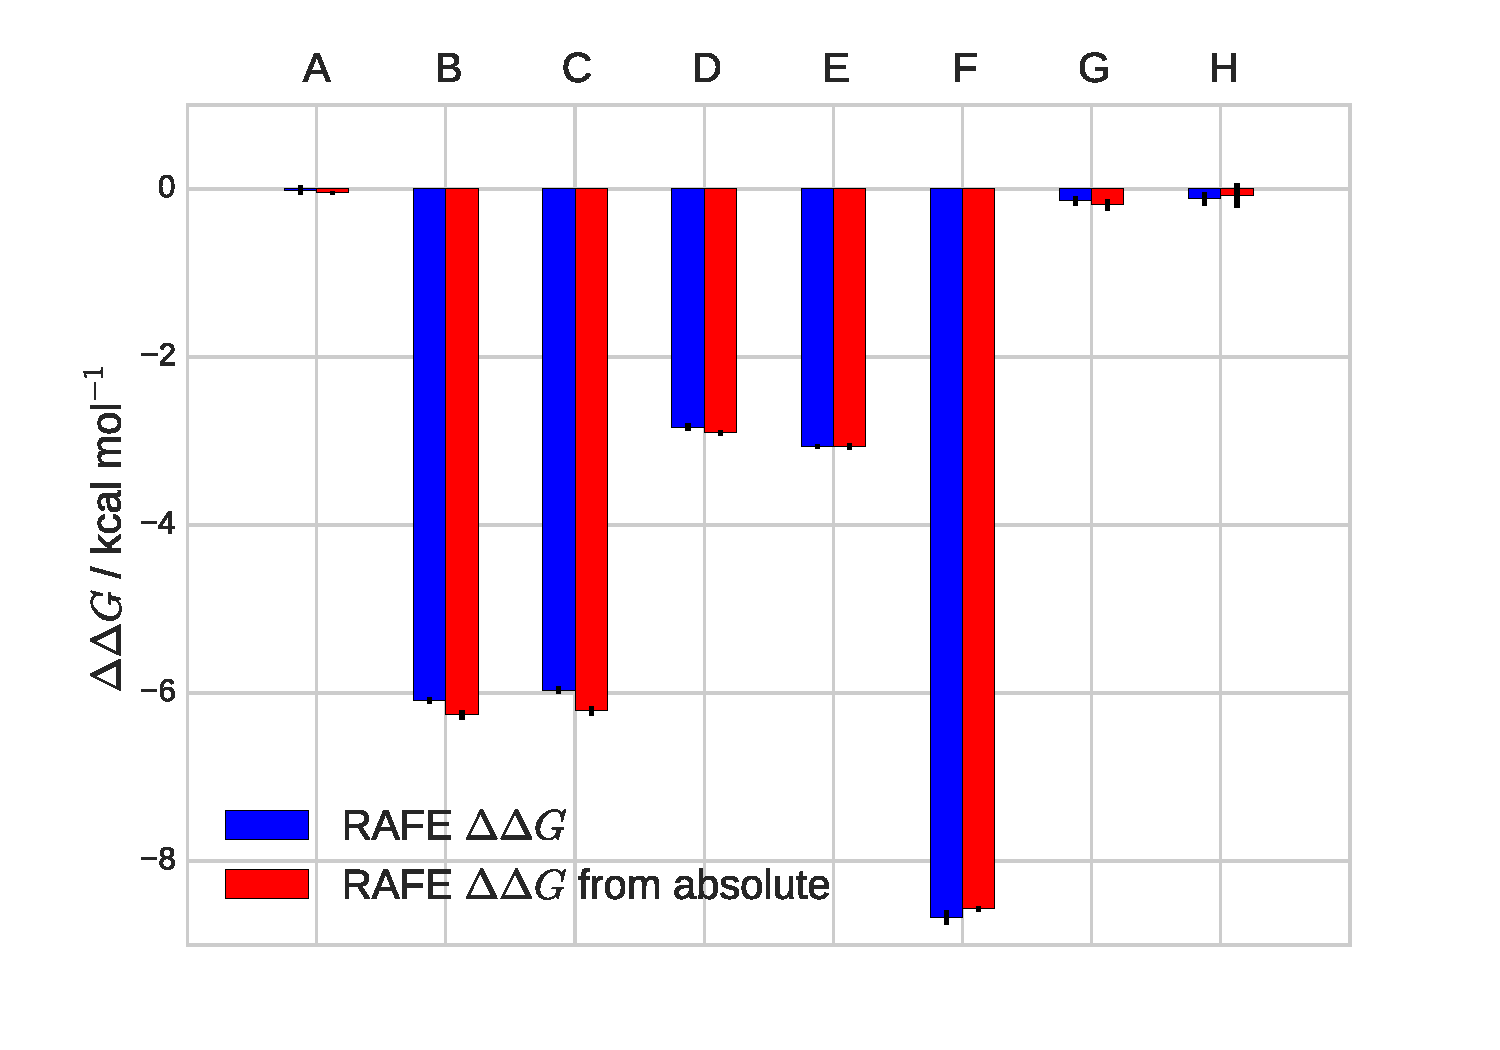
\includegraphics[width=\textwidth]{figures/sire_histogram.pdf}
  \caption{Relative free energy of hydration $\Delta\Delta G$, computed with 
  RAFE calculations, compared with $\Delta\Delta G$ derived from absolute free 
  energy calculations for A: methane to ethane, B: ethane to methanol, C: 
  methane to methanol, D: methane to 2-methylfuran, E: methane to toluene,
    F: methane to 2-methylindole, G: methane to neopentane, H: 
    2-cyclopentanylindole to 7-cyclopentanylindole.}
  \label{fig:sire_histogram}
\end{figure}

\todo{we could write a 95\% confidence interval MUE: \SI{0.08}< \SI{0.11} < 
\SI{0.14}{kcal.mol^{-1}}}

To achieve reproducibility in Sire/SOMD and among all the other codes, the role 
of constraints was crucial and a new kind of constraint was employed: 
unperturbed hydrogen bond constraint. Here, all the unperturbed hydrogen 
atoms'bonds are constrained, while the perturbed hydrogen atoms, namely atoms 
which undergo a transformation, are unconstrained and their masses are
equal to the heavier mass of the two end states. In this way symmetry between 
forward and backward transformations is guaranteed, and a time step of 
\SI{2}{fs} can be employed.

\todo{maybe add figure to SI explaining how these constraints are used}

This new constraint overcomes issues encountered with Sire/SOMD starting 
protocol.
% halx: what is the ``starting protocol''
Usually, RAFE calculations were performed with all bonds constrained, 
in order to have time step longer than \SI{2}{fs}~\cite{hopkins2015long},
% halx: really longer than 2fs
enhancing sampling with a reasonable computational cost.
However, from a technical point of view, a constraint in Sire/SOMD sets the 
bond energy to zero.  This may be a valid approximation for small and rigid 
molecules, but a systematic offset is introduced which necessarily increases 
with every additional perturbation introduced.
%DLM: I don't understand the "a systematic offset" part here.
Indeed, looking at neopentane $\rightarrow$ methane (centrally mapped) this 
bias gives a RAFE $\Delta\Delta G$=\SI{2.04 +- 0.01}{kcal.mol^{-1}} in contrast 
to $\Delta G$=\SI{-0.19+-0.06}{kcal.mol^{-1}} from the absolute calculations, 
as tab.~\ref{S-tab:sire_constraints} and fig.~\ref{S-fig:sire_constraints} show.
Furthermore, neopentane $\rightarrow$ methane (terminally mapped) shows a 
$\Delta\Delta G$ =\SI{0.59 +- 0.01}{kcal.mol^{-1}}. As the free energy must be 
independent of the chosen path this discrepancy denotes a problem with using 
constraints on transformed atoms. 
This problem has been discussed by Pearlman~\cite{pearlman1991overlooked} 
and Boresch~\cite{doi:10.1021/jp981628n, doi:10.1021/jp981629f}, 
as a missing bond-stretching term, which can be estimated as: 
\begin{equation}
 \label{eq:allbondserror}
 \Delta G= RT\ln \left ( \frac{r_{\mathrm{i}}}{r_\mathrm{f}} \right)  
\end{equation}
where $r_{\mathrm{i}}$ and $r_{\mathrm{f}}$ are the initial and final bond 
lengths, respectively.  Although for small bond length changes this error may 
be negligible, it becomes pivotal for perturbations of hydrogen atoms to 
carbon, nitrogen or oxygen, where the bond length changes of several tenths of 
an \AA.
% halx: please quantify

After the implementation of the our new constraint scheme, a comparison with simulations without constraints has been run. 
Figure~\ref{S-fig:sire_constraints} shows 
that both protocols attain the same results with a final 
MUE = \SI{0.09}{kcal.mol^{-1}}.

% halx: we don't have MUE for the other results so need to discuss if we want 
%       to use this
%       most of the following needs to be discussed at the beginning of this 
%c      chapter when comparing all codes
Tab~\ref{tab:mue-comp} shows the MUE between Sire/SOMD, Gromacs employing 
%DLM: Should be GROMACS, not Gromacs, throughout (it's an acronym, like AMBER)
%DLM: Also should be AMBER throughout.
reaction field (Gromacs RF), Gromacs with PME (Gromacs PME) and Amber  
(alternatively: Tab~\ref{tab:muebound-comp} shows the MUE comparison with 
95$\%$ of confidence interval between Sire/SOMD, Gromacs with reaction 
field (Gromacs RF), Gromacs with PME (Gromacs PME) and Amber). 
As regards reaction field methods, Sire/SOMD implements a Barker Watts reaction 
% halx: citation for BWRF missing
field (BWRF) with a atom based cutoff, as explained in 
subsection~\ref{sec:rafe_protocols}, while Gromacs adopts a BWRF with a
charge group cutoff.  Despite this technical difference,
Sire/SOMD and Gromacs RF produce comparable results with a MUE of 
\SI{0.18}{kcal.mol^{-1}}.
In]the methane $\rightarrow$ neopentane transformation is still matter of 
problems. In this case, Sire/SOMD is able to maintain consistency between 
central and terminal mapping, as shown in tab~\ref{S-tab:sire-finalresults}, 
while Gromacs RF displays a $\Delta\Delta$G of \SI{-0.20 +- 
0.01}{kcal.mol^{-1}} for the
centrally mapped transformation and $\Delta\Delta$G = \SI{-0.05 +- 
0.02}{kcal.mol^{-1}} for the terminally mapped transformation.
As regards PME methods, Sire/SOMD presents a MUE = \SI{0.18}{kcal.mol^{-1}} and 
MUE = \SI{0.23}{kcal.mol^{-1}} with Gromacs PME and Amber respectively, 
achieving a very good agreement between $\Delta\Delta$G predictions. 

\todo{it may be good to say somewhere how much was the MUE with the initial 
standard protocol} %DLM: What is "initial standard protocol"?

\todo{Gromacs RF in vacuum uses a dielectric of 1.0, this causes problems for 
Sire vacuum simulations} %DLM: What does this mean? 

Overall, the Sire/SOMD free energy estimations are in good agreement with the 
other MD packages, as the MUE suggests.  Reaction field and PME results are in 
good agreement.  In particular, the unperturbed hydrogen bonds constraint 
%DLM: "unperturbed hydrogen bonds constraint" is unclear.
allows a timestep of \SI{2}{fs} and Sire/SOMD RAFE simulations can be carried 
out in one 
single step.


\begin{table}[]
  \begin{minipage}{\linewidth}
  \caption{MUE comparison between Sire/SOMD, Gromacs with Reaction Field (Gromacs RF), Gromacs with PME (Gromacs PME) and Amber in terms of MUE (\SI{}{kcal.mol^{-1}}.}\label{tab:mue-comp}
  \makebox[\textwidth][c]{
  \begin{tabular}{lrrrr}
    \toprule
    Package & Sire/SOMD & Gromcs RF & Gromacs PME & Amber\\
    \midrule
Sire/SOMD         & 0.00 & 0.18    & 0.18 & 0.23\\
Gromacs RF   & 0.18 & 0.00    & 0.04 & 0.14\\ 
Gromacs PME  & 0.18 & 0.04    & 0.00 & 0.14\\     
Amber        & 0.23 & 0.14    & 0.14 & 0.00\\
     \bottomrule
  \end{tabular}
}
  \end{minipage}
\end{table}


\begin{table}[]
  \begin{minipage}{\linewidth}
  \caption{MUE with 95$\%$ confidence interval between Sire/SOMD, Gromacs with Reaction Field (Gromacs RF), Gromacs with PME (Gromacs PME) and Amber in terms of MUE (\SI{}{kcal.mol^{-1}}.}\label{tab:muebound-comp}
  \makebox[\textwidth][c]{
  \begin{tabular}{lcccc}
    \toprule
    Package & Sire/SOMD & Gromcs RF & Gromacs PME & Amber\\
    \midrule
Sire/SOMD         & 0.02< 0.04< 0.05 & 0.17< 0.19< 0.21    & 0.16< 0.18< 0.20 & 0.21< 0.23< 0.25\\
Gromacs RF   	  & 0.17< 0.18< 0.19 & 0.01< 0.02< 0.03    & 0.04< 0.05< 0.06 & 0.13< 0.14< 0.15\\
Gromacs PME       & 0.17< 0.18< 0.19 & 0.04< 0.05< 0.06    & 0.01< 0.02< 0.03 & 0.14< 0.15< 0.16\\
Amber		  & 0.22< 0.23< 0.24 & 0.13< 0.14< 0.15    & 0.14< 0.15< 0.16 & 0.01< 0.02< 0.03\\
     \bottomrule
  \end{tabular}
}
  \end{minipage}
\end{table}


\section{Discussion}
\label{sec:discuss}

\todo{recommended protocols}

\todo{protocols to avoid}

\todo{lessons learned}

\todo{2-cyclopentanylindole to 7-cyclopentanylindole: better to go through intermediates?}

\todo{%
 what do we need to progress the field e.g. automation to make things
 easy but also consistent and thus more reproducible (FESetup also
 for reproducibility); GPU: Gromacs, SOMD but not AMBER (yet) and
 CHARMM; alternative softcore functions?; sampling?; force field improvements?; analysis?
}

\todo{%
 developer notes: constraints, both appearing/disappearing;
 lambda paths for AMBER (relative), absolute: crgmask requires
 vacuum corr if separated protocol
}

\todo{further investigation required: binding RAFEs?}


\listoftodos


\begin{acknowledgement}
  HHL is supported through an EPSRC provided SLA, funding the core
  support of CCPBioSim.  CCPBioSim is the Collaborative Computational
  Project for Biomolecular Simulation funded by EPSRC grants
  EP/J010588/1 and EP/M022609/1.  JM is supported by a Royal Society
  University Research Fellowship.  The research leading to these
  results has received funding from the European Research Council
  under the European Unions Seventh Framework Programme
  (FP7/2007--2013)/ERC Grant agreement No.\ 336289.  GDRM appreciates
  the support from the Brazilian agency CAPES - Science without
  Borders program (BEX 3932-13-3).  DLM appreciates support from the
  National Science Foundation (CHE 1352608), and computing support
  from the UCI GreenPlanet cluster, supported in part by NSF Grant
  CHE-0840513.

  We thank Prof.\ Stefan Boresch for valuable discussions and making code
  modifications to CHARMM.  We thank Dr.\ Ross Walker and Daniel Mermelstein
  for valuable discussions and making code modifications to AMBER.  We thank
  Prof. Michael Shirts for valuable discussions about Gromacs.

  We acknowledge use of Hartree Centre resources and the use of the
  SCARF HPC cluster in this work.
\end{acknowledgement}

% \begin{suppinfo}
% \end{suppinfo}

\bibliography{journal-abbrev,reprod}

\end{document}

%  LocalWords:  loeffler
